\documentclass[11pt]{article}

\usepackage[margin=1in]{geometry}
\usepackage{tikz}
\usetikzlibrary{shapes.geometric, arrows.meta, positioning, shapes.misc}
\usepackage{enumitem}
\usepackage{titlesec}
\usepackage{hyperref}
\usepackage{xcolor}
\usepackage{booktabs}

\hypersetup{colorlinks=true, linkcolor=blue, urlcolor=blue}

\titleformat{\section}{\normalfont\Large\bfseries}{\thesection}{1em}{}
\titleformat{\subsection}{\normalfont\large\bfseries}{\thesubsection}{1em}{}

\title{\textbf{StitchPerfect}\\[4pt]\large Revolutionizing Tailor Shops}
\author{Uday Singh \\ Roll No.: 1024160031}
\date{}

\begin{document}

\maketitle
\vspace{-1em}
\begin{center}
\textit{Digitize Orders \quad Precision Measurements \quad Faster Deliveries \quad Data-Driven Growth}
\end{center}

\section*{Problem Statement Title}
Enhancing Tailor Shop Efficiency through Digital Management and Automation.

\section{Higher-order Goal}
Local tailor shops largely depend on manual, paper-based processes for taking measurements,
tracking orders, and coordinating with staff. This leads to measurement errors, long turnaround
times, and missed business opportunities. StitchPerfect aims to digitize order intake, standardize
measurement storage, and provide real-time visibility into shop operations for both staff and
customers, reducing rework and improving delivery speed.

\section{Problem Statement}
People running or working in local tailor shops routinely face avoidable inefficiencies caused by
manual record-keeping:

\begin{itemize}[leftmargin=1.5em]
  \item \textbf{Measurement mistakes:} measurements recorded on paper are easy to misplace, misread, or lose between visits.
  \item \textbf{Long turnarounds:} lack of a structured order pipeline makes it difficult to track where a garment is in the stitching process.
  \item \textbf{Lost sales:} without visibility into inventory and order status, shops struggle to manage repeat customers and growth.
  \item \textbf{No customer visibility:} customers have no way to track their order or verify progress before collection.
  \item \textbf{Fragmented staff coordination:} new staff onboarding is slow, and task assignment across workers is informal.
\end{itemize}

\noindent\textbf{Why this matters:} A digital, tailor-first platform that standardizes measurements and
automates the order workflow can materially reduce errors and delivery time while giving shop
owners the operational visibility needed to scale.

\section{Proposed Solution}

\subsection{Overview}
StitchPerfect is a digital management platform built specifically for tailor shops and boutiques.
Rather than being a generic order-tracking tool, it combines measurement digitization,
media-based proof-of-work, inventory tracking, and customer communication into a single
tailor-first system.

The proposed solution consists of the following components:

\begin{itemize}[leftmargin=1.5em]
  \item \textbf{Order Management \& Workflow:} digital order intake, task cards, and status
        tracking through the full stitching pipeline.
  \item \textbf{Media Management (Cloudinary):} photo-based proof-of-work, style references,
        and design previews stored in the cloud.
  \item \textbf{Inventory \& Material Tracking:} real-time fabric and material stock control
        linked to active orders.
  \item \textbf{Customer Communication \& Payments:} automated updates, reminders, and
        integrated payment collection.
  \item \textbf{Measurement Explorer:} centralized, searchable storage of customer measurement
        profiles for faster reorders.
  \item \textbf{Worker Console:} task queues and status updates for stitching staff.
  \item \textbf{Admin Panel:} full operational oversight of orders, workers, and delivery status,
        with support for multi-shop, role-based access.
\end{itemize}

\subsection{How this solves the problem}
By digitizing measurements, automating the order workflow, and providing customer-facing
tracking with backend analytics, StitchPerfect reduces rework caused by lost or miscommunicated
measurements, shortens lead times through clearer task ownership, and increases shop revenue by
enabling faster repeat orders and better inventory decisions.

\subsection{Who benefits}
\begin{itemize}[leftmargin=1.5em]
  \item \textbf{Tailors \& stitching staff:} simpler daily queues, clear task cards, fewer
        corrections, saved measurement profiles, faster onboarding.
  \item \textbf{Shops \& owners:} visibility into all orders, cost and profitability per garment,
        inventory control, supplier integration, scalability to multiple outlets.
  \item \textbf{Customers:} order tracking, preview images, fewer fittings, trusted
        proof-of-work, faster delivery and easier reorders.
  \item \textbf{Suppliers \& vendors:} electronic purchase orders, lead-time tracking, demand
        forecasts from analytics.
  \item \textbf{Investors / business partners:} monetization metrics, growth projections, low
        customer acquisition cost via shop partnerships.
\end{itemize}

\section{System Context Diagram}
Figure~\ref{fig:context} provides a high-level view of StitchPerfect and its interaction with the
primary external actors: customers, tailoring staff, shop owners/administrators, and suppliers.
This places the StitchPerfect platform at the center, unifying the tailoring value chain into a
single digital system.

\begin{figure}[h!]
\centering
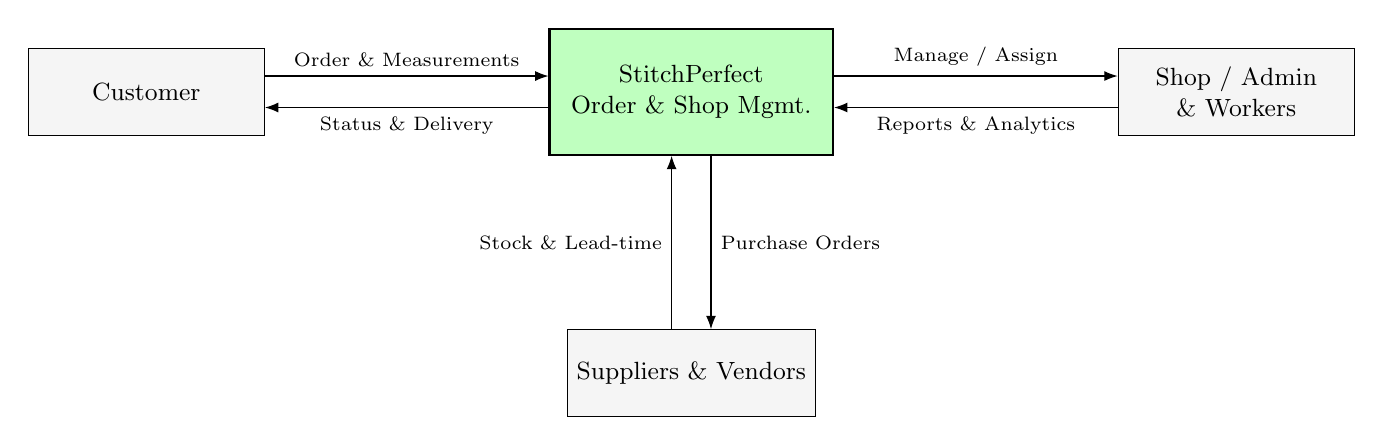
\begin{tikzpicture}[
  node distance=3.6cm,
  box/.style={rectangle, draw, minimum width=3cm, minimum height=1.1cm, align=center, fill=gray!8, font=\small},
  core/.style={rectangle, draw, minimum width=3.6cm, minimum height=1.6cm, align=center, fill=green!25, thick, font=\small},
  >=Latex
]
\node[core] (sp) {StitchPerfect\\Order \& Shop Mgmt.};
\node[box, left=of sp] (cust) {Customer};
\node[box, right=of sp] (admin) {Shop / Admin\\\& Workers};
\node[box, below=2.2cm of sp] (sup) {Suppliers \& Vendors};

\draw[->] ([yshift=0.2cm]cust.east) -- node[midway, above, font=\scriptsize] {Order \& Measurements} ([yshift=0.2cm]sp.west);
\draw[->] ([yshift=-0.2cm]sp.west) -- node[midway, below, font=\scriptsize] {Status \& Delivery} ([yshift=-0.2cm]cust.east);

\draw[->] ([yshift=0.2cm]sp.east) -- node[midway, above, font=\scriptsize] {Manage / Assign} ([yshift=0.2cm]admin.west);
\draw[->] ([yshift=-0.2cm]admin.west) -- node[midway, below, font=\scriptsize] {Reports \& Analytics} ([yshift=-0.2cm]sp.east);

\draw[->] ([xshift=0.25cm]sp.south) -- node[midway, right, font=\scriptsize] {Purchase Orders} ([xshift=0.25cm]sup.north);
\draw[->] ([xshift=-0.25cm]sup.north) -- node[midway, left, font=\scriptsize] {Stock \& Lead-time} ([xshift=-0.25cm]sp.south);
\end{tikzpicture}
\caption{Level-0 Context Diagram for StitchPerfect}
\label{fig:context}
\end{figure}

\section{Use Case Diagram}
Figure~\ref{fig:usecase} illustrates the major functional interactions between customers,
tailoring staff/workers, and shop administrators.

\begin{figure}[h!]
\centering
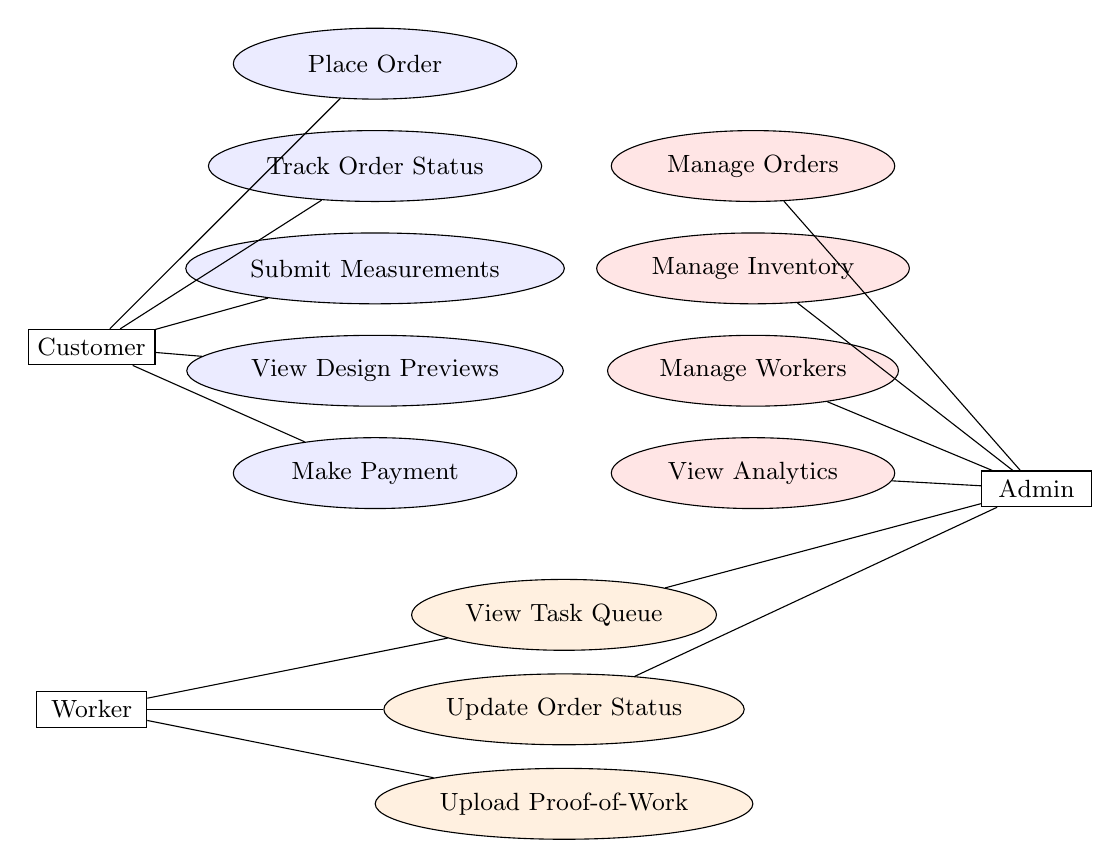
\begin{tikzpicture}[
  actor/.style={draw, minimum width=1.4cm, align=center, font=\small},
  uc/.style={ellipse, draw, minimum width=3.6cm, minimum height=0.9cm, align=center, font=\small, fill=blue!8},
  ucw/.style={ellipse, draw, minimum width=3.6cm, minimum height=0.9cm, align=center, font=\small, fill=orange!12},
  uca/.style={ellipse, draw, minimum width=3.6cm, minimum height=0.9cm, align=center, font=\small, fill=red!10},
  >=Latex
]

\node[actor] (customer) at (0,-3.6) {Customer};
\node[actor] (worker) at (0,-8.2) {Worker};
\node[actor] (admin) at (12,-5.4) {Admin};

\node[uc] (place)   at (3.6,0)    {Place Order};
\node[uc] (track)   at (3.6,-1.3)   {Track Order Status};
\node[uc] (measure) at (3.6,-2.6)   {Submit Measurements};
\node[uc] (view)    at (3.6,-3.9)   {View Design Previews};
\node[uc] (pay)     at (3.6,-5.2)   {Make Payment};

\node[uca] (manage) at (8.4,-1.3)   {Manage Orders};
\node[uca] (inv)    at (8.4,-2.6)   {Manage Inventory};
\node[uca] (workers)at (8.4,-3.9)   {Manage Workers};
\node[uca] (anal)   at (8.4,-5.2)   {View Analytics};

\node[ucw] (queue)  at (6,-7)   {View Task Queue};
\node[ucw] (update) at (6,-8.2)   {Update Order Status};
\node[ucw] (upload) at (6,-9.4)   {Upload Proof-of-Work};

\draw (customer) -- (place);
\draw (customer) -- (track);
\draw (customer) -- (measure);
\draw (customer) -- (view);
\draw (customer) -- (pay);

\draw (worker) -- (queue);
\draw (worker) -- (update);
\draw (worker) -- (upload);

\draw (admin) -- (manage);
\draw (admin) -- (inv);
\draw (admin) -- (workers);
\draw (admin) -- (anal);
\draw (admin) -- (queue);
\draw (admin) -- (update);

\end{tikzpicture}
\caption{Use Case Diagram for StitchPerfect}
\label{fig:usecase}
\end{figure}

\section{Level-1 Data Flow Diagram}
Figure~\ref{fig:dfd} expands the system context into the main functional processes and data
stores within StitchPerfect. Process 6.0 (Customer Comm.\ \& Payments) is also responsible for
pushing status updates and reminders back out to the customer, alongside the direct order and
measurement intake shown at process 1.0.

\begin{figure}[h!]
\centering
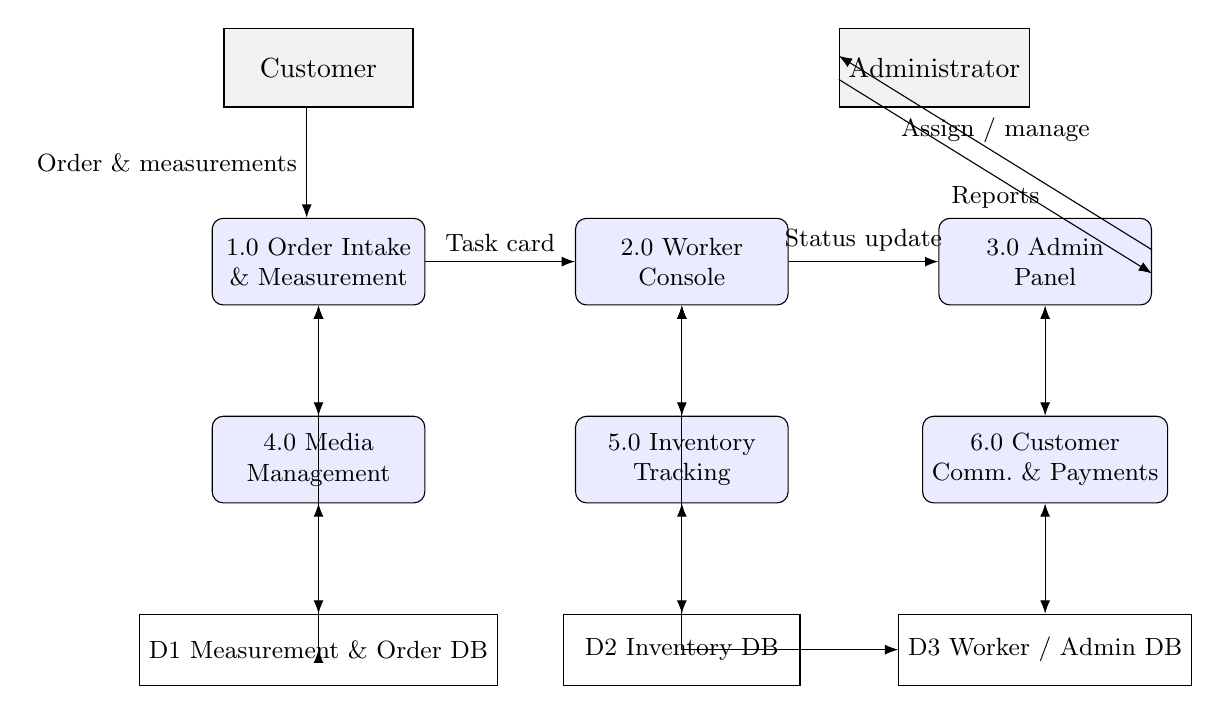
\begin{tikzpicture}[
  node distance=1.6cm and 1.9cm,
  ext/.style={rectangle, draw, minimum width=2.4cm, minimum height=1cm, align=center, fill=gray!10},
  proc/.style={rectangle, rounded corners, draw, minimum width=2.7cm, minimum height=1.1cm, align=center, fill=blue!8, font=\small},
  store/.style={rectangle, draw, minimum width=3cm, minimum height=0.9cm, align=center, font=\small},
  >=Latex
]

\node[ext] (cust) {Customer};
\node[ext, right=5.4cm of cust] (admin) {Administrator};

\node[proc, below=1.4cm of cust] (order) {1.0 Order Intake\\\& Measurement};
\node[proc, right=1.9cm of order] (worker) {2.0 Worker\\Console};
\node[proc, right=1.9cm of worker] (mgmt) {3.0 Admin\\Panel};

\node[proc, below=1.4cm of order] (media) {4.0 Media\\Management};
\node[proc, below=1.4cm of worker] (invp) {5.0 Inventory\\Tracking};
\node[proc, below=1.4cm of mgmt] (comm) {6.0 Customer\\Comm.\ \& Payments};

\node[store, below=1.4cm of media] (d1) {D1 Measurement \& Order DB};
\node[store, below=1.4cm of invp] (d2) {D2 Inventory DB};
\node[store, below=1.4cm of comm] (d3) {D3 Worker / Admin DB};

\draw[->] ([xshift=-0.15cm]cust.south) -- node[midway, left, font=\small] {Order \& measurements} ([xshift=-0.15cm]order.north);
\draw[->] (order) -- node[midway, above, font=\small] {Task card} (worker);
\draw[->] (worker) -- node[midway, above, font=\small] {Status update} (mgmt);
\draw[->] ([yshift=0.15cm]mgmt.east) -- node[midway, above, font=\small] {Assign / manage} ([yshift=0.15cm]admin.west);
\draw[<-] ([yshift=-0.15cm]mgmt.east) -- node[midway, below, font=\small] {Reports} ([yshift=-0.15cm]admin.west);

\draw[<->] (order) -- (media);
\draw[<->] (worker) -- (invp);
\draw[<->] (mgmt) -- (comm);

\draw[<->] (media) -- (d1);
\draw[<->] (order) |- (d1);
\draw[<->] (invp) -- (d2);
\draw[<->] (comm) -- (d3);
\draw[<->] (worker) |- (d3);

\end{tikzpicture}
\caption{Level-1 Data Flow Diagram for StitchPerfect}
\label{fig:dfd}
\end{figure}

\section{Solution Approach}

\subsection{Implementation flow}
The administrator signs in to a central Admin Panel that branches into the Worker Console and
Measurement Explorer, and further into Order Delivery, Ready Products, and the Worker List,
giving full operational control over daily shop activity.

\subsection{Technology stack}
StitchPerfect is built on a lightweight, scalable stack:
\begin{itemize}[leftmargin=1.5em]
  \item \textbf{Bootstrap} -- responsive front-end UI.
  \item \textbf{Node.js} -- backend server.
  \item \textbf{jQuery} -- dynamic front-end interactivity.
  \item \textbf{Cloudinary} -- media and image management (proof-of-work, style references).
  \item \textbf{Aiven} -- managed cloud database infrastructure.
\end{itemize}

\subsection{Database design}
The schema centers on the \texttt{mesurement} table, which records every order and links back to
\texttt{customerlist} (via mobile number) and \texttt{workerlist} (via worker name) -- a
one-to-many relationship in both cases, since a single customer can place many orders and a
single worker can be assigned to many orders. The \texttt{pass} table stores admin login
credentials independently of the order data.

\begin{center}
\begin{tabular}{@{}ll@{}}
\toprule
\textbf{Table} & \textbf{Key} \\
\midrule
\texttt{customerlist} & PK: \texttt{mobile} \\
\texttt{workerlist} & PK: \texttt{wname} \\
\texttt{mesurement} & PK: \texttt{orderid}; FK: \texttt{mobile} $\to$ \texttt{customerlist.mobile}; FK: \texttt{worker} $\to$ \texttt{workerlist.wname} \\
\texttt{pass} & PK: \texttt{id} (standalone, no foreign keys) \\
\bottomrule
\end{tabular}
\end{center}

\subsection{Ecosystem}
The StitchPerfect platform sits at the center of the tailoring ecosystem, connecting tailoring
staff, shop owners, and customers on one side with suppliers, investors, and multi-shop operators
on the other -- unifying the entire tailoring value chain into a single digital system, and
supporting multi-shop management with role-based access as the platform scales.

\end{document}
